\chapter{Design and Implementation}

\section{Architecture design}

%-----------This is a FIGURE-----------------------
\begin{figure}[htbp]
	\centering
	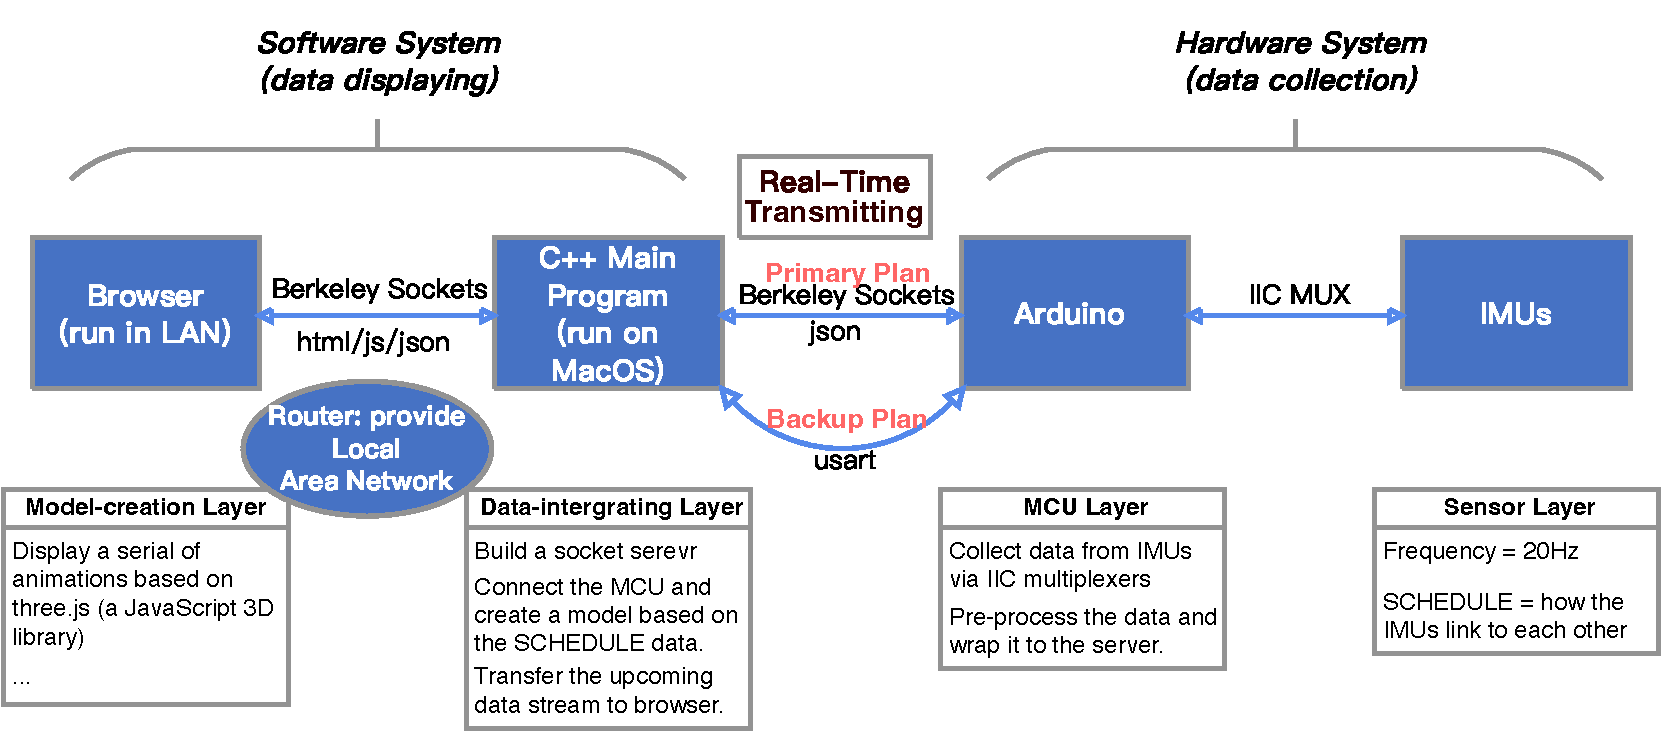
\includegraphics[clip, trim=0cm 0cm 0cm 0cm, width=1\textwidth]{
		fileForWriting/sketch_map}
	\caption[Project architecture diagram]{Project architecture diagram. }
	\label{fig:project-architecture-diagram}
\end{figure}
%--------End of this FIGURE -----------  

In order to ensure efficient task allocation, the project was partitioned into two modules as Figure~\ref{fig:project-architecture-diagram} has shown: hardware and software.
The hardware module was delegated to three MRS students, based on their respective areas of expertise and preferences.
Their responsibilities encompassed the utilization of Arduino to collect data from multiple sensors through an IIC multiplexer, and an implementation of WiFi data transmission.
Additionally, a backup plan utilizing wired communication through USART was selected, considering the development timeline and difficulty of wireless communication.

On the other hand, the software module was entrusted to two CSEE students.
The responsibilities of the two CSEE students encompassed two tasks.
The first one is to construct a simple C++ socket server to function as the data center.
Secondly, they were tasked with developing a rudimentary human lower limb model using Three.js, an external JavaScript graphic library.

Upon achieving these objectives, users would be able to access the visualized digital twin directly through a web browser with ease.
To facilitate debugging, the entire network would operate within a local area network (LAN). However, it could be expanded to the internet in the future.

\section{Real-time rendering design}
%-----------This is a FIGURE-----------------------
\begin{figure}[htbp]
	\centering
	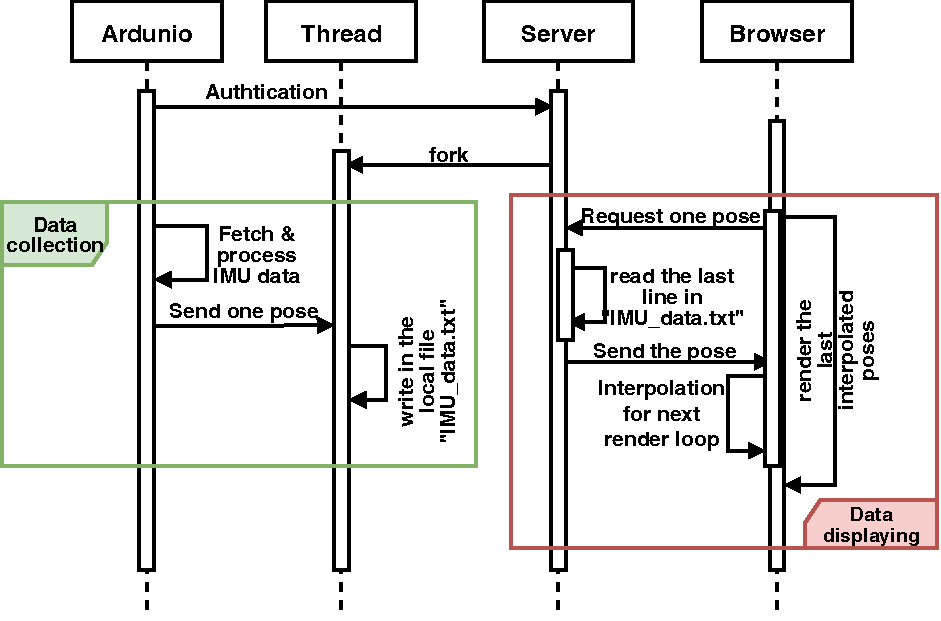
\includegraphics[clip, trim=0cm 0cm 0cm 0cm, width=\textwidth]{
		fileForWriting/sequence}
	\caption[Transmitting logic of motion data]{Transmitting logic of motion data collected by IMUs, where a single pose represents data from four IMUs, two each from the femur and tibia.}
	\label{fig:sequence}
\end{figure}
%--------End of this FIGURE -----------
In this project, real-time rendering is designated as a potentially critical task metric.
To achieve such functionality, two key steps are thus implemented.
The first step is to ensure that the front-end could access the latest motion data.
On the server, a thread is dedicated to continuously writing motion data from the IMU to the same text file.
As the left hand side of Data-displaying loop in Figure~\ref{fig:sequence} may illustrate, once the front-end browser request a pose data, another thread of server will be launched to read the last line of the txt file and send it back to the client.

The second operation aims to reduce wireless communication latency.
In the displaying engine, multi-threading is also employed.
One thread is specifically designed to render the animation, while another is responsible for requesting data from the server and interpolating the returned data for use in the next rendering.
This approach will not only smooth the animation but also offset some latency caused by communication delays.

\section{3D model design}

%-----------This is a FIGURE-----------------------
\begin{figure}[htbp]
	\centering
	\includegraphics[width=\textwidth]{
		fileForWriting/3d-model}
	\caption[Model for holding an IMU on the femur]{Model for holding an IMU on the femur (rendered by SolidWorks Software).}
	\label{fig:3d-model}
\end{figure}
%--------End of this FIGURE -----------  


The IMU-holding component for the femur and tibia has been designed with a flat top edge and a curved bottom edge, as shown in Figure~\ref{fig:3d-model}.
It conforms precisely to the curve of the human leg, resulting in a more comfortable fit.
To minimize shock and vibration to IMU during testing, a form tape has been added into the designated IMU slot.
Additionally, adjustable VELCRO straps have been incorporated into the component to accommodate different leg sizes, ensuring ease and speed of use.

Furthermore, two protective techniques have been employed to prevent damage to the data cable during testing.
Firstly, a spiral wrap has been added to the data cable to provide additional protection.
Finally, each component has been perforated with holes, through which a hemp rope has been threaded to prevent external forces from dislodging the cable.
